\chapter{High Availability and Resolver Agent Deployments}
\label{sec:high-availability}

\section{Overview}

\cxoneflow can be deployed in a high-availability configuration using multiple instances of
the \cxoneflow container.  The \cxoneflow instances need to have a shared MQ cluster that
can communicate with the AMQP protocol.  The MQ instance is where long-running state data
is persisted by each instance.  Figure \ref{fig:ha-diagram} shows a deployment diagram for
a typical high-availability configuration.


\begin{figure}[h]
    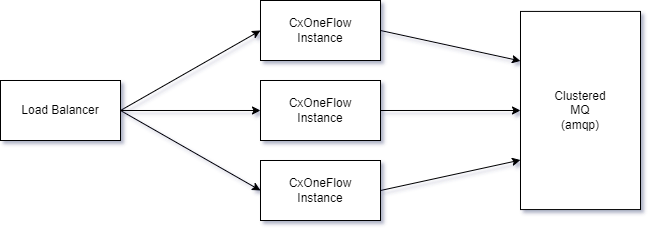
\includegraphics[width=\textwidth]{graphics/cxoneflow-diagrams-HA.png}
    \caption{High Availability Deployment Diagram}
    \label{fig:ha-diagram}
\end{figure}


\section{Load Balancing \cxoneflow Endpoints}

A typical load balancer round-robin configuration can be used to load balance \cxoneflow endpoint container instances.
There is no user interface component to \cxoneflow; this means that each connection to the \cxoneflow endpoint is stateless
and will not require any session-affinity (aka sticky-sessions) settings on the load balancer.

The \texttt{/ping} endpoint on the \cxoneflow container can be used for health-check by the load balancer.  
It is recommended that all instances of the \cxoneflow endpoint containers are using the same version.

Multiple \cxoneflow endpoint containers behind a load balancer is recommended but not technically required
when deploying \hyperref[sec:resolver-agent]{resolver agents}.  However, an external message queue shared by the \cxoneflow endpoints
and the resolver agent instances is required to distribute resolver scan jobs and results.  

\section{External Message Queue}

An external message queue is required for high-availability deployments of \cxoneflow or deployments that use distributed
\hyperref[sec:resolver-agent]{resolver agents}.  Although a single instance of an external message queue can be used, it is
recommended that the external message queue use a clustered configuration for purposes of high-availability.  The message queue
must understand the AMQP protocol and be able to implement the concepts of Topic Exchanges, replicated queues, and queue
dead-letter exchanges.  While there may be many message queue servers that understand AMQP, the recommended message queue
server is RabbitMQ.\footnote{The "Amazon MQ Service" in AWS can be used to easily deploy a managed RabbitMQ cluster.}

It is highly recommended to create a \textbf{non-administrative} message queue user for use in the \cxoneflow endpoint
connection configuration.  The user account connected to the MQ must have the ability to configure the
exchange and queue schema.  The user permissions configuration may vary by message queue platforms; the user permissions
needed when using RabbitMQ can be found in Table \ref{tab:server-mq-user-perms}.  

Note that the permissions in Table \ref{tab:server-mq-user-perms} are not the same permissions
that should be applied in \hyperref[sec:resolver-agent]{resolver agent} configurations; please see Chapter \ref{sec:resolver-agent} for more
information about message queue user permissions for resolver agents.

\begin{table}[ht]
    \caption{RabbitMQ User Permissions for the \cxoneflow Endpoint}  
    \label{tab:server-mq-user-perms}      
    \begin{tabularx}{\textwidth}{lcl}
        \toprule
        \textbf{Permission} & \textbf{Regular Expression} \\
        \midrule
        \texttt{Configure} & \texttt{\^{}cx:.*} \\
        \midrule
        \texttt{Write} & \texttt{\^{}cx:.*} \\
        \midrule
        \texttt{Read} & \texttt{\^{}cx:.*} \\
        \midrule
        \bottomrule
    \end{tabularx}
\end{table}



